\chapter{Neural Net Implementation} \label{chap:kitt_nn}
Plenty of neural network implementations are available nowadays. Nevertheless, one of the objectives of this thesis is to implement own framework capable of using the idea behind artificial feedforward neural networks. Besides prooving a knowledge of mathematical and algorithmical backgrounds, an integration of own utilities and functions is the main reason for the from-scratch implementation.

To accomplish the reasearch objectives, the new framework must meet following requirements, which might be unusal for some of the provided implementations (mentioned in \cref{chapter:01:state_of_the_art}).

\begin{itemize}
\item ability to remove any synapse in a network and then to retrain the network of the new structure
\item ability to evaluate a network after each learning epoch and basically to provide an open-sourced learning algorithm
\item ability to illustrate a network structure and to visualize the learning process in real time (an extra property)
\end{itemize}

In this thesis, the implemented neural network framework is called \textbf{kitt\_nn} and has been developed in programming language Python. The following diagram (\ref{img:kitt_nn_package}) shows the structure of the \textit{kitt\_nn .py package}.

\begin{figure}[H]
  \centering
  \includegraphics[width=0.75\textwidth]{kitt_nn_package.png}
  \caption{kitt\_nn package : Implemented neural network framework}
  \label{img:kitt_nn_package}
\end{figure}

Moreover, the framework must have some standard functions implemented, meaning it must be capable of:

\begin{itemize}
\item initializing a feedforward network of any structure supplied by some randomly set parameters
\item fitting a model to a network (function \textit{fit()}), training a network on some data of a conventional structure
\item predicting a target of never-seen samples (function \textit{predict()}), evaluating a classification performance
\end{itemize}

The \textit{kitt\_nn} implementation is based on some general knowledge gained at school and/or from [], the idea is pretty straight forward.

\section{Structural Elements}
The overall idea is based on the object-oriented programming. There are three main \textit{.py} files containing the main classes corresponding to strucutural elements - a network, a neuron and a synapse (a connection). A detailed API is attached as an appendix (\ref{app:code_documentation}).

\subsection*{kitt\_neuron.py} \label{ssec:kitt_neuron}
The very basic units of a neural net are called neurons. In case of artificial systems, these units are responsible for transfering all their inputs into one output. The behavior is moreless the same for all of the units, therefore a class called \textit{Neuron} implements some basic common functions.

\begin{figure}[H]
  \centering
  \includegraphics[width=0.6\textwidth]{kitt_neuron.png}
  \caption{kitt\_neuron.py : Neuron class inheritance}
  \label{img:kitt_neuron}
\end{figure}

Then, as \cref{img:kitt_neuron} shows, three classes are inherited from the \textit{Neuron} class. Some special functions, depending on the layer a neuron is part of, can be implemented this way.

\subsection*{kitt\_synapse.py} \label{ssec:kitt_synapse}
Next, there is a class representing a neural connection - a synapse. An instance of this class takes care of the corresponding weight and remembers the two connected neurons. 

Additionally, a function called \textbf{remove\_self()} is implemented, which sets the weight to zero and removes the synapse from all databases of the corresponding neural net. Then it also checks the two connected neurons, if they have some other connections remaining. If not, they are labeled as \textit{dead}, as they are not a part of the network anymore.

\subsection*{kitt\_net.py} \label{ssec:kitt_net}
The network is initialized by creating an instance of \textit{NeuralNetwork()} class from \textit{kitt\_net.py}. The initialization process is illustrated in \cref{img:kitt_net}. Basically, the only parameter is the network structure, which is expected as a \textit{.py iterable} type. For instance, a network with 2 input, 5 hidden and 3 output units would be created as \textit{NeuralNetwork(structure=[2, 5, 3])}. Number of hidden layers is not limited.

\begin{figure}[H]
  \centering
  \includegraphics[width=0.7\textwidth]{kitt_net.png}
  \caption{kitt\_net.py : Neural Network Initialization}
  \label{img:kitt_net}
\end{figure}

A learning algorithm is added to the initialized network thereafter (see \cref{sec:learning_algorithm}). The network class implements basic functions like \textit{fit()}, \textit{predict()} in order to be used as a classifier. Moreover, it has some additional utilities like \textit{copy\_self()} or \textit{print\_self()}, which are essential for this research (\cref{sec:gui}, \cref{sec:network_pruning_algorithm}).

\section{Learning Algorithm} \label{sec:learning_algorithm}
Backpropagation implementation in python

algorithm

1-2 pages

\section{Graphical User Interface} \label{sec:gui}
The graphical interface has been implemented as an extension for \textit{kitt\_nn} framework. It is actually not strictly needed for this research, but it provides some interesting functions, which are worth of being introduced. Anyway, any type of visualization usually helps to understand a problem better.

\begin{figure}[H]
  \centering
  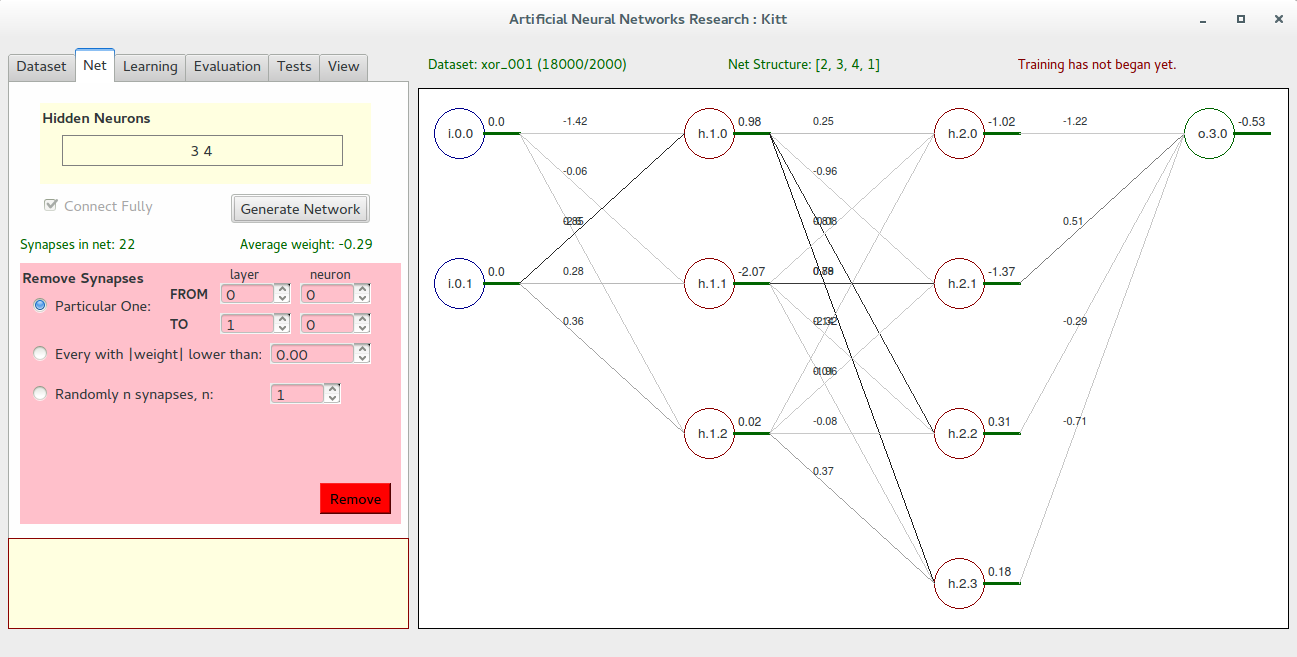
\includegraphics[width=1.0\textwidth]{gui_screen.png}
  \caption{Screenshot of the graphical user interface}
  \label{img:gui_screen}
\end{figure}

This GUI is capable of:
\begin{enumerate}
\item Loading a dataset in a specific form and, if possible, visualizing it (see XOR data in \cref{img:data_xor} for an example, this image is generated by the GUI).
\item Generating a network of any hidden structure. The input and output layers are defined by the chosen dataset. The network is then visualized (as shown in \cref{img:gui_screen}).
\item Removing synapses of the network, while the visualization is interactive with the structure changes.
\item Training the network, while the visualization is interactive, so the weights changes can be seen online.
\item Performing some tests and plotting simple evaluations.
\item Adjusting the visualization view in sense of zooming, resizing or changing colors.
\end{enumerate}

The visualization is not that useful for huge network structures, however, it can be essential at some points of the research. Nevertheless, it is considered as the very fist version for now and aimed to be upgraded in the future.

\newpage
\section{Network Pruning Algorithm} \label{sec:network_pruning_algorithm}

\begin{figure}[H]
  \centering
  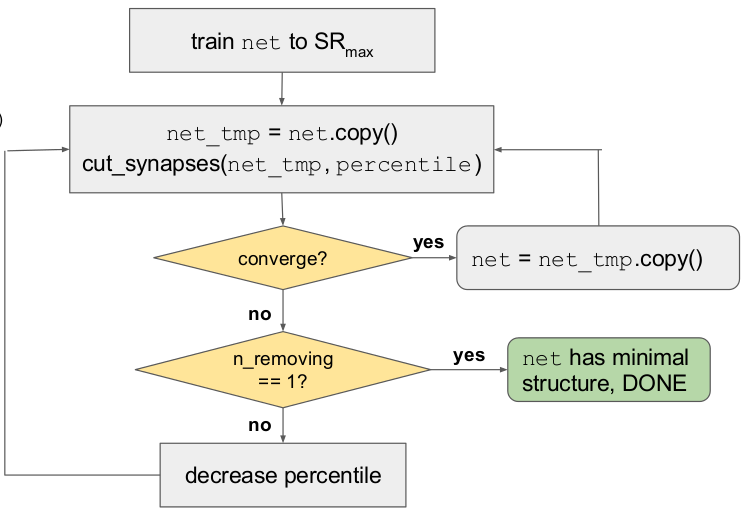
\includegraphics[width=1.0\textwidth]{pruning_algorithm.png}
  \caption{The Pruning Algorithm}
  \label{img:pruning_algorithm}
\end{figure}

\subsection{Testing Datasets}

\subsubsection*{XOR Dataset}

\begin{figure}[H]
  \centering
  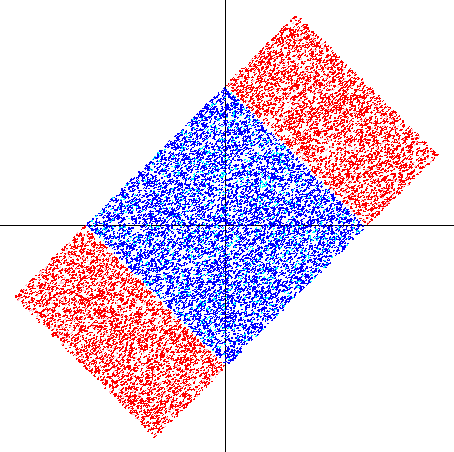
\includegraphics[width=0.7\textwidth]{data_xor.png}
  \caption{2D XOR Data illustration}
  \label{img:data_xor}
\end{figure}

\begin{figure}[H]
  \centering
  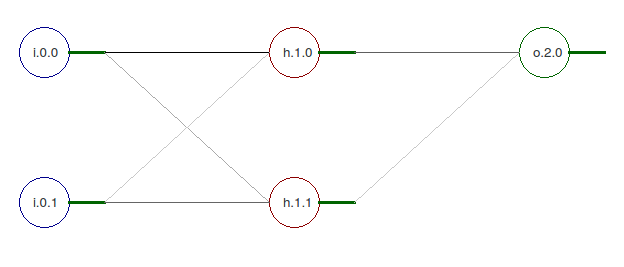
\includegraphics[width=0.6\textwidth]{xor_min_structure_1.png}
  \caption{XOR min structure 1}
  \label{img:xor_min_structure_1}
\end{figure}

\begin{figure}[H]
  \centering
  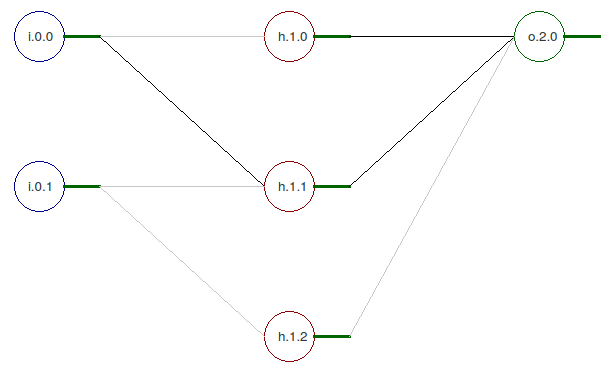
\includegraphics[width=0.6\textwidth]{xor_min_structure_2.png}
  \caption{XOR min structure 2}
  \label{img:xor_min_structure_2}
\end{figure}

\subsubsection*{MNIST Dataset}

\begin{figure}[H]
  \centering
  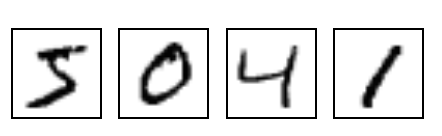
\includegraphics[width=0.7\textwidth]{data_mnist.png}
  \caption{MNIST Data illustration}
  \label{img:data_mnist}
\end{figure}

\subsection{Minimal Structures Utilization}
further MNIST analysis

figures, tables

4-5 pages